\documentclass[12pt]{article}
\usepackage{geometry}                % See geometry.pdf to learn the layout options. There are lots.
\geometry{letterpaper}                   % ... or a4paper or a5paper or ... 
\usepackage{graphicx}
\usepackage{amssymb}
\usepackage{amsthm}
\usepackage{epstopdf}
\usepackage[utf8]{inputenc}
\usepackage[usenames,dvipsnames]{color}
\usepackage[table]{xcolor}
\usepackage{hyperref}
\DeclareGraphicsRule{.tif}{png}{.png}{`convert #1 `dirname #1`/`basename #1 .tif`.png}

\theoremstyle{definition}
\newtheorem{example}{Example}

\newenvironment{explanation}{%
   \setlength{\parindent}{0pt}
   \itshape
   \color{blue}
}{}

\newcommand{\projectname}{PanSim}
\newcommand{\productname}{Pandemic Simulator}
\newcommand{\projectleader}{O. Dominik}
\newcommand{\documentstatus}{In process}
%\newcommand{\documentstatus}{Submitted}
%\newcommand{\documentstatus}{Released}
\newcommand{\version}{V. 1.0}

\begin{document}
\begin{titlepage}
\begin{flushright}

\includegraphics[scale=.5]{htlleondinglogo.png}\\
\end{flushright}

\vspace{10em}

\begin{center}
{\Huge Project Proposal} \\[3em]
{\LARGE \productname} \\[3em]
\end{center}

\begin{flushleft}
\begin{tabular}{|l|l|}
\hline
Project Name & \projectname \\ \hline
Project Leader & \projectleader \\ \hline
Document state & \documentstatus \\ \hline
Version & \version \\ \hline
\end{tabular}
\end{flushleft}

\end{titlepage}
\section*{Revisions}
\begin{tabular}{|l|l|l|}
\hline
\cellcolor[gray]{0.5}\textcolor{white}{Date} & \cellcolor[gray]{0.5}\textcolor{white}{Author} & \cellcolor[gray]{0.5}\textcolor{white}{Change} \\ \hline
November 03, 2011&P. Bauer/T. Stütz&First version \\ \hline
\end{tabular}
\pagebreak

\tableofcontents
\pagebreak

\section{Introduction}

Our team decided to simulate a pandemic to help contain future panedemics more swiftly.
During the current corona crisis it has become apparent that we need some way to predict the direction of a pandemic.
In terms of feasebility we would first simulate a virus with just numbers and no graphical elements but later on we will incorperate a GUI if it is necessary.
Since this is a purely scientific simulation done by students affordability and market and economic efficiency can not be determined.
Since there isn't any funding involved in this project there are no risks only opportunities.


\pagebreak

\section{Initial Situation}

The current corona crisis has shown us that an pandemic cannot be foreseen and needs to be dealt with as fast as possible in order to stop its spread.
Currently measures like masks, shields or curfews cannot be tested unless they have shown some effect to stop the spread of a virus.
We looked at a few diffrent simulations that try to predict the future of a pandemic.

Epimath Austria is a simulation of the corona pendamic in austria. The data is shown in multiple understandable graphs and seems quite exact for the time it takes to compute.
As already mentioned Epimath only simulates the corona pandamic so it is not possible to simulate any other viruses.
Also it does not have the possability to add or remove savety measures or vaccines.

The pandemic simulation from janarosmonaliev at SUNY Korea simulates a city with people in it that infect others on contact.
You can change and view all the settings but while watching the simulation i couldn't see anyone new getting infected.

\pagebreak

\section{General Conditions and Constraints}

Our data needs to be obtained through trustworthy sources like government websites, universities etc.
This includes data on the virus as well as how to simulate viruses.
If we arent able to do that the whole simulation will give imprecise and false results.
So it is very necessary to get our informations from officaly and trustworthy sources. 

Also we currently lack the expertise to do such simulations which means we need to do some research first.
Otherwise we only create a simulation of how we think a simulation works and not how it should really work based on real data, events, etc.

The only tool we can currently use are our own laptops which means the simulation can't be too complex so that it doesn't run on these devices.
(Change the Constraint and put it in risks)

\pagebreak

\section{Project Objectives and System Concepts}

Our results shall be presented as clear and easy readable as possible, 
that means that data like infectionsrate, susceptible, infected, casualties and recovered should be displayed on a graph.
Calculations of the virus shall reflect a real and clear scenario with as much precision as possible.
Therefore all initial data for the virus, event probability, etc. must be displayed.

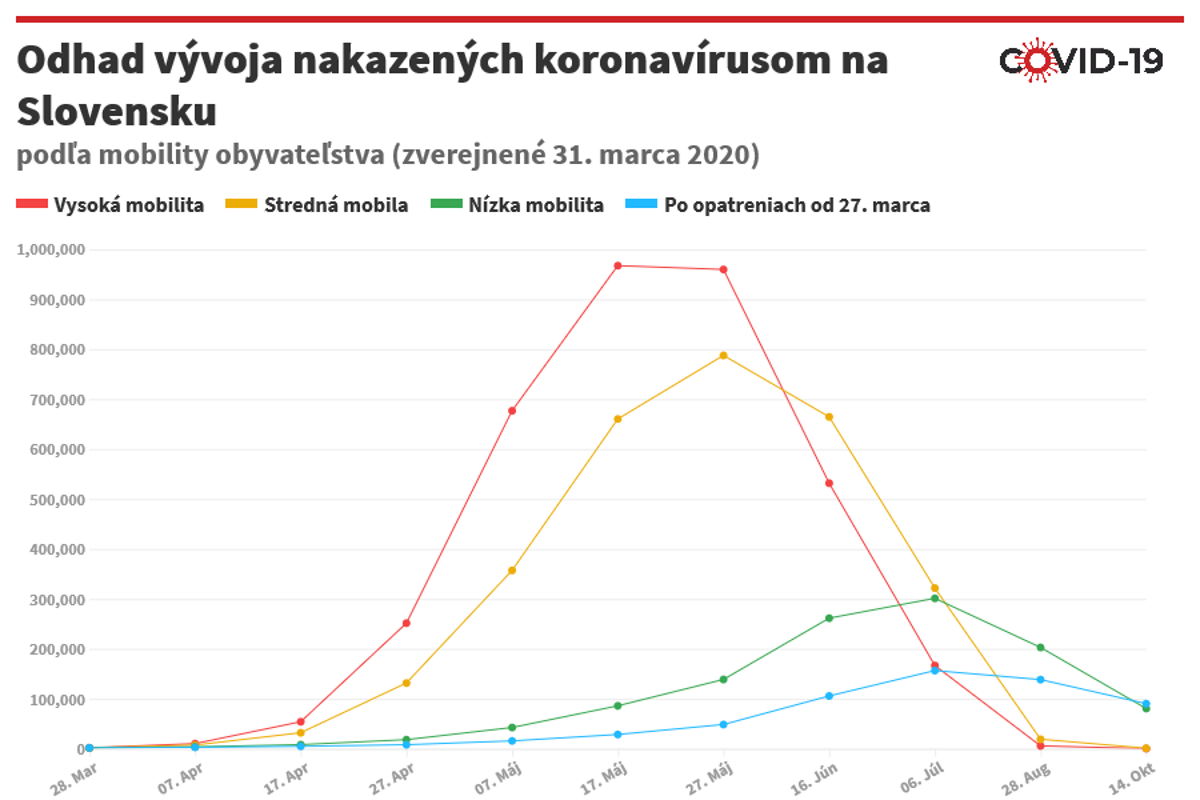
\includegraphics[width=\textwidth]{graph.png}\\[2em]
Here you can see corona graph of Slovenia in this way we want to show our calculated data. Every colored line stands for a differnet sector.

For example: blue for recovered, red for deaths and yellow for current infections.

\pagebreak
\section{Opportunities and Risks}

The first and most obvious opportunity is that we can predict current and future pandemics and therefore act swifter and more precise.
Building up from there we plan on displaying the results in a way that is easily readable for everyone so that it can be used as a proper source.

Because of the high attention this project will receive due to corona it shall be communicated very well at public events of the HTL Leonding.
The government will probably see these presentations and maybe support our project with data and/or hardware.

We can run into the risk that our simulations get too complex and we run out of computing power.
Also we don't yet know how to simulate a virus and therefore don't know how long it will take us.

\pagebreak
\section{Planning}

The first step to complete this project will be create a list of features that the simulation shall have. 
We will collect all knowledge about the mathmatics of a pandemic that is necessary to implement those features and edit the list so that all the features are possible to implement in the given time.
As a Deadline for this step we will set january 14th. 

After that we will start with the actual programming.
The first simple prototype should be ready by feburary 4th. After that we will need another week to implement a graph with the results that the prototype put out.


At this point we will start adding features from our list. On May 16th our simualtion should be ready test using real life pandemics. 
We will be doing this by trying to recreate real life pandemics and compareing the simulated data with the actual data.


If there is still some time left we will use it to implement an easy to understand graphical user interface.

\end{document}  